\documentclass{ci5652}
\usepackage{graphicx,amssymb,amsmath}
\usepackage[utf8]{inputenc}
\usepackage[spanish]{babel}
\usepackage{hyperref}
\usepackage{subfigure}
\usepackage{paralist}
\usepackage[ruled,vlined,linesnumbered]{algorithm2e}

%----------------------- Macros and Definitions --------------------------

% Add all additional macros here, do NOT include any additional files.

% The environments theorem (Theorem), invar (Invariant), lemma (Lemma),
% cor (Corollary), obs (Observation), conj (Conjecture), and prop
% (Proposition) are already defined in the ci5652.cls file.

\graphicspath{ {plots/} }

%----------------------- Title -------------------------------------------

\title{Problema de selección de prototipo (IS/PS):\\
       Un enfoque con metaheurísticas}

\author{Juan Carlos Arocha Ovalles
        \and
        Matteo José Ferrando Briceño}

%------------------------------ Text -------------------------------------

\begin{document}
\thispagestyle{empty}
\maketitle


\begin{abstract}
El uso de clasificadores para determinar la clase de algún \textit{documento} está intimamente relacionado con el conjuntos de datos \textit{TR} con el que son entrenados. Un TR que represente adecuadamente a la muestra contiene potencialmente una gran cantidad de instancias, lo que genera un entrenamiento y una clasificación lenta. El objetivo de este estudio es encontrar, haciendo uso de metaheurísticas, un subconjunto de TR considerablemente más pequeño que mantenga el mismo desempeño de clasificación.

Entre las metaheurísticas probadas, tenemos Búsqueda Local, Búsqueda Local Iterada, GRASP y algoritmos evolutivos como GGA (Algoritmo Genético Generacional) y SGA (Algoritmo Genético Estacionario), y  dentro de ellas, se hizo uso de una función objetivo exponencial que prioriza la clasificación sobre la reducción para comparar soluciones y de una perturbación inteligente, la cual prioriza aquellos puntos que potencialmente mejoren más la solución.

XXX INSERTAR RESUMEN DE RESULTADOS XXX
XXX INSERTAR RESUMEN DE CONCLUSIONES XXX


\end{abstract}

\section{Problema de selección de prototipo}

En el campo de clasificación de documentos, la calidad de clasificadores como \textit{K-NN} depende del TR con el cual sean entrenados. Un problema que se encuentra a la hora de elegir el TR es la selección de las intancias que lo conforman. Una gran cantidad instancias que representen las diferentes clases, pueden llevar a una buena clasificación, pero a su vez llevan a un entrenamiento y a un desempeño lento por parte de los clasificadores.

Es por ello que se ha intentado reducir este conjunto para disminuir el tiempo de entrenamiento y clasificación, pero manteniendo la calidad de los resultados que se obtengan.

Este problema es bastante común en diversas áreas de ciencias de la computación, por ejemplo, procesamiento y etiquetado de imágenes, análisis de \textit{big data}, análisis de lenguaje natural, \textit{Data Mining}, entre otros por lo que ha sido bastante estudiado y existen diversas soluciones propuestas.

\section{Trabajos anteriores}
\label{sect:works}

Entre las soluciones que se estudiaron en el estado del arte, en~\cite{toussaint2002proximity} Toussaint describe soluciones de tipo \textit{Greedy} como CNN, RNN y MCNN, las cuales demuestran una baja complejidad de tiempo y cuyos resultados son aceptables pero no optimales.Cano y Herrera en ~\cite{1255391}, proponen utiliazr algoritmos evolutivos solucionar el problema de selección de instancias para extracción de conocimientos en bases de datos (KDD), presentan una función de evaluación de calidad que se utilizaron para las pruebas; finalmente, concluyen que para KDD, los algoritmos evolutivos mejoran tanto la reducción del subconjunto, como la presición. Luego García y Derrac, con apoyo de Cano y Herrera, en ~\cite{garcia2012prototype} hacen un análisis extenso de los diversos algritmos basados en el algoritmo \textit{K-NN}.

\section{Metaheurísticas}
\label{sect:meta}

Como se vió en~\cite{1255391}, una forma de resolver el problema IS/PS es usando metaheurísticas. Una metaheurística es un método genérico de solución de problemas computacionales, que no toma en cuenta el enunciado del problema sino la representación de sus soluciones, para luego mejorarlas en un tiempo eficiente pero que no asegura la optimalidad.

La mayoría de las metaheurísticas parten de una solución inicial, y a través de métodos iterativos, mejoran dicha solución, manteniendo la mejor de todas vista hasta el momento. La condición de parada de las mismas suelen variar entre un límite de tiempo, de iteraciones o que el espacio de búsqueda no provea mejores soluciones.

Para poder realizar pruebas usando metaheurísticas, se necesita una representación de la solución del problema planteado. En este caso, IS/PS fue representado con un conjunto \textbf{SP} que corresponde a las instancias que se encuentran dentro del subconjunto de TR seleccionado y el resto de los puntos se encuentra en el conjunto \textbf{UP}. Por otro lado, también es necesario tener una funcion que sea capaz de evaluar una solución y que de este modo dos soluciones sean comparables. Como se vió en la sección~\ref{sect:works}, la calidad del subconjunto de TR seleccionado depende de la calidad de clasificación y del tamaño del mismo. La calidad se puede representar como el porcentaje de documentos bien clasificados, y el tamaño como el porcentaje de reducción de TR, lo que genera una función con dos variables. Para los experimentos se propusieron tres funciones:

\begin{equation}\label{eq:weight}
f(cl,rd) = \alpha\times cl + (1 - \alpha)\times rd
\end{equation}

\begin{equation}\label{eq:sqr}
f(cl,rd) = (cl + (1 - \alpha))^{2}\times (rd + \alpha)^{2}
\end{equation}

\begin{equation}\label{eq:exp}
f(cl,rd) = \beta^{(cl + (1 - \alpha))\times (rd + \alpha)}
\end{equation}

Donde $cl$ corresponde al porcentaje de classificación correcta, $rd$ al porcentaje de reducción de TR, $\alpha$ al peso en porcentaje (entre 0 y 1) que tiene $cl$ con respecto a $rd$ y $\beta$ a un número real arbitrario. La razón por la cual de toman estas funciones es porque se busca penalizar la puntuación obtenida por las mismas cuando cualquier de los dos atributos, sea $cl$ o $rd$, tengan valores muy bajos.

Por otra parte, también es necesario definir un operador de vecindad, el cual consiste en una función capaz de generar nuevas soluciones a partir de cualquier solución. El mismo depende de la metaheurística aplicada a problema.

En los experimentos realizados en este estudio, se consideró el uso de búsqueda local como metaheurística lineal y búsqueda local iterada y GRASP como metaheurísticas de trayectoria.

% FIGURA DE FUNCIÓN POR PESO
\begin{figure}[p]
    \centering
    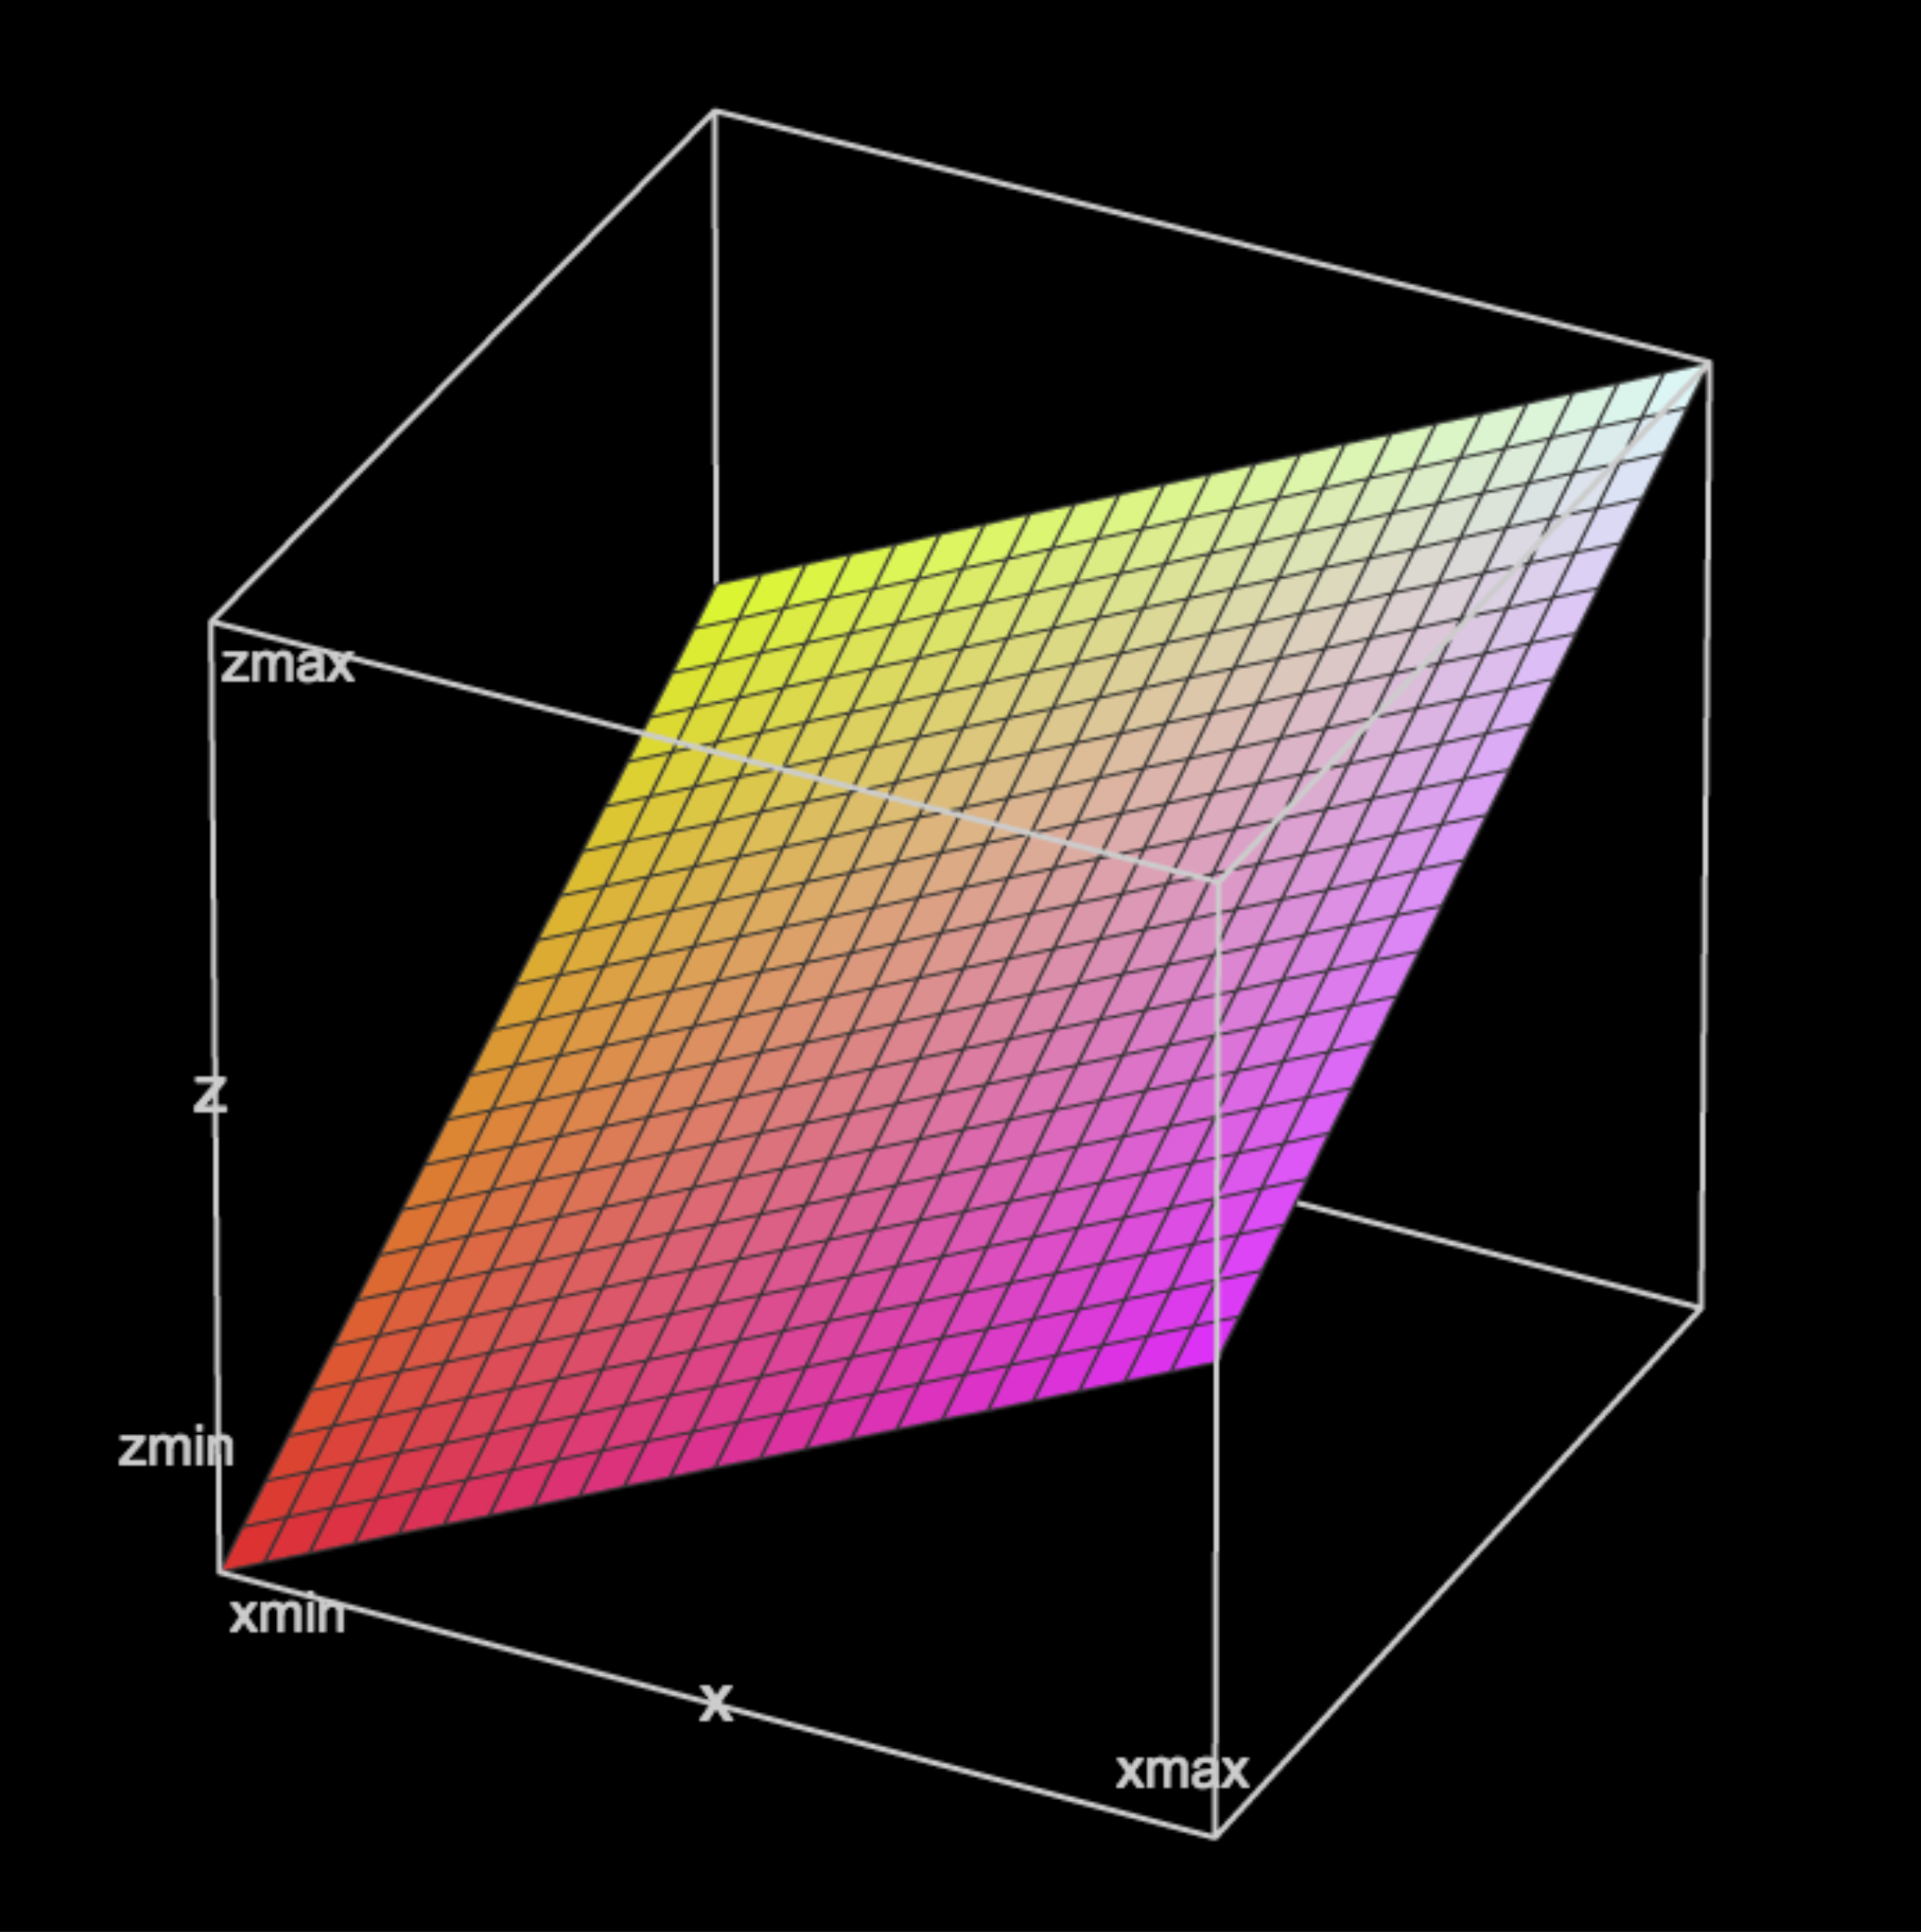
\includegraphics[width=0.8\linewidth]{weighted-3b}
    \caption{Función planar, ecuación~\ref{eq:weight}}
    \label{fig:weighted3}
\end{figure}

% FIGURA DE FUNCIÓN CUADRÁTICA
\begin{figure}[p]
    \centering
    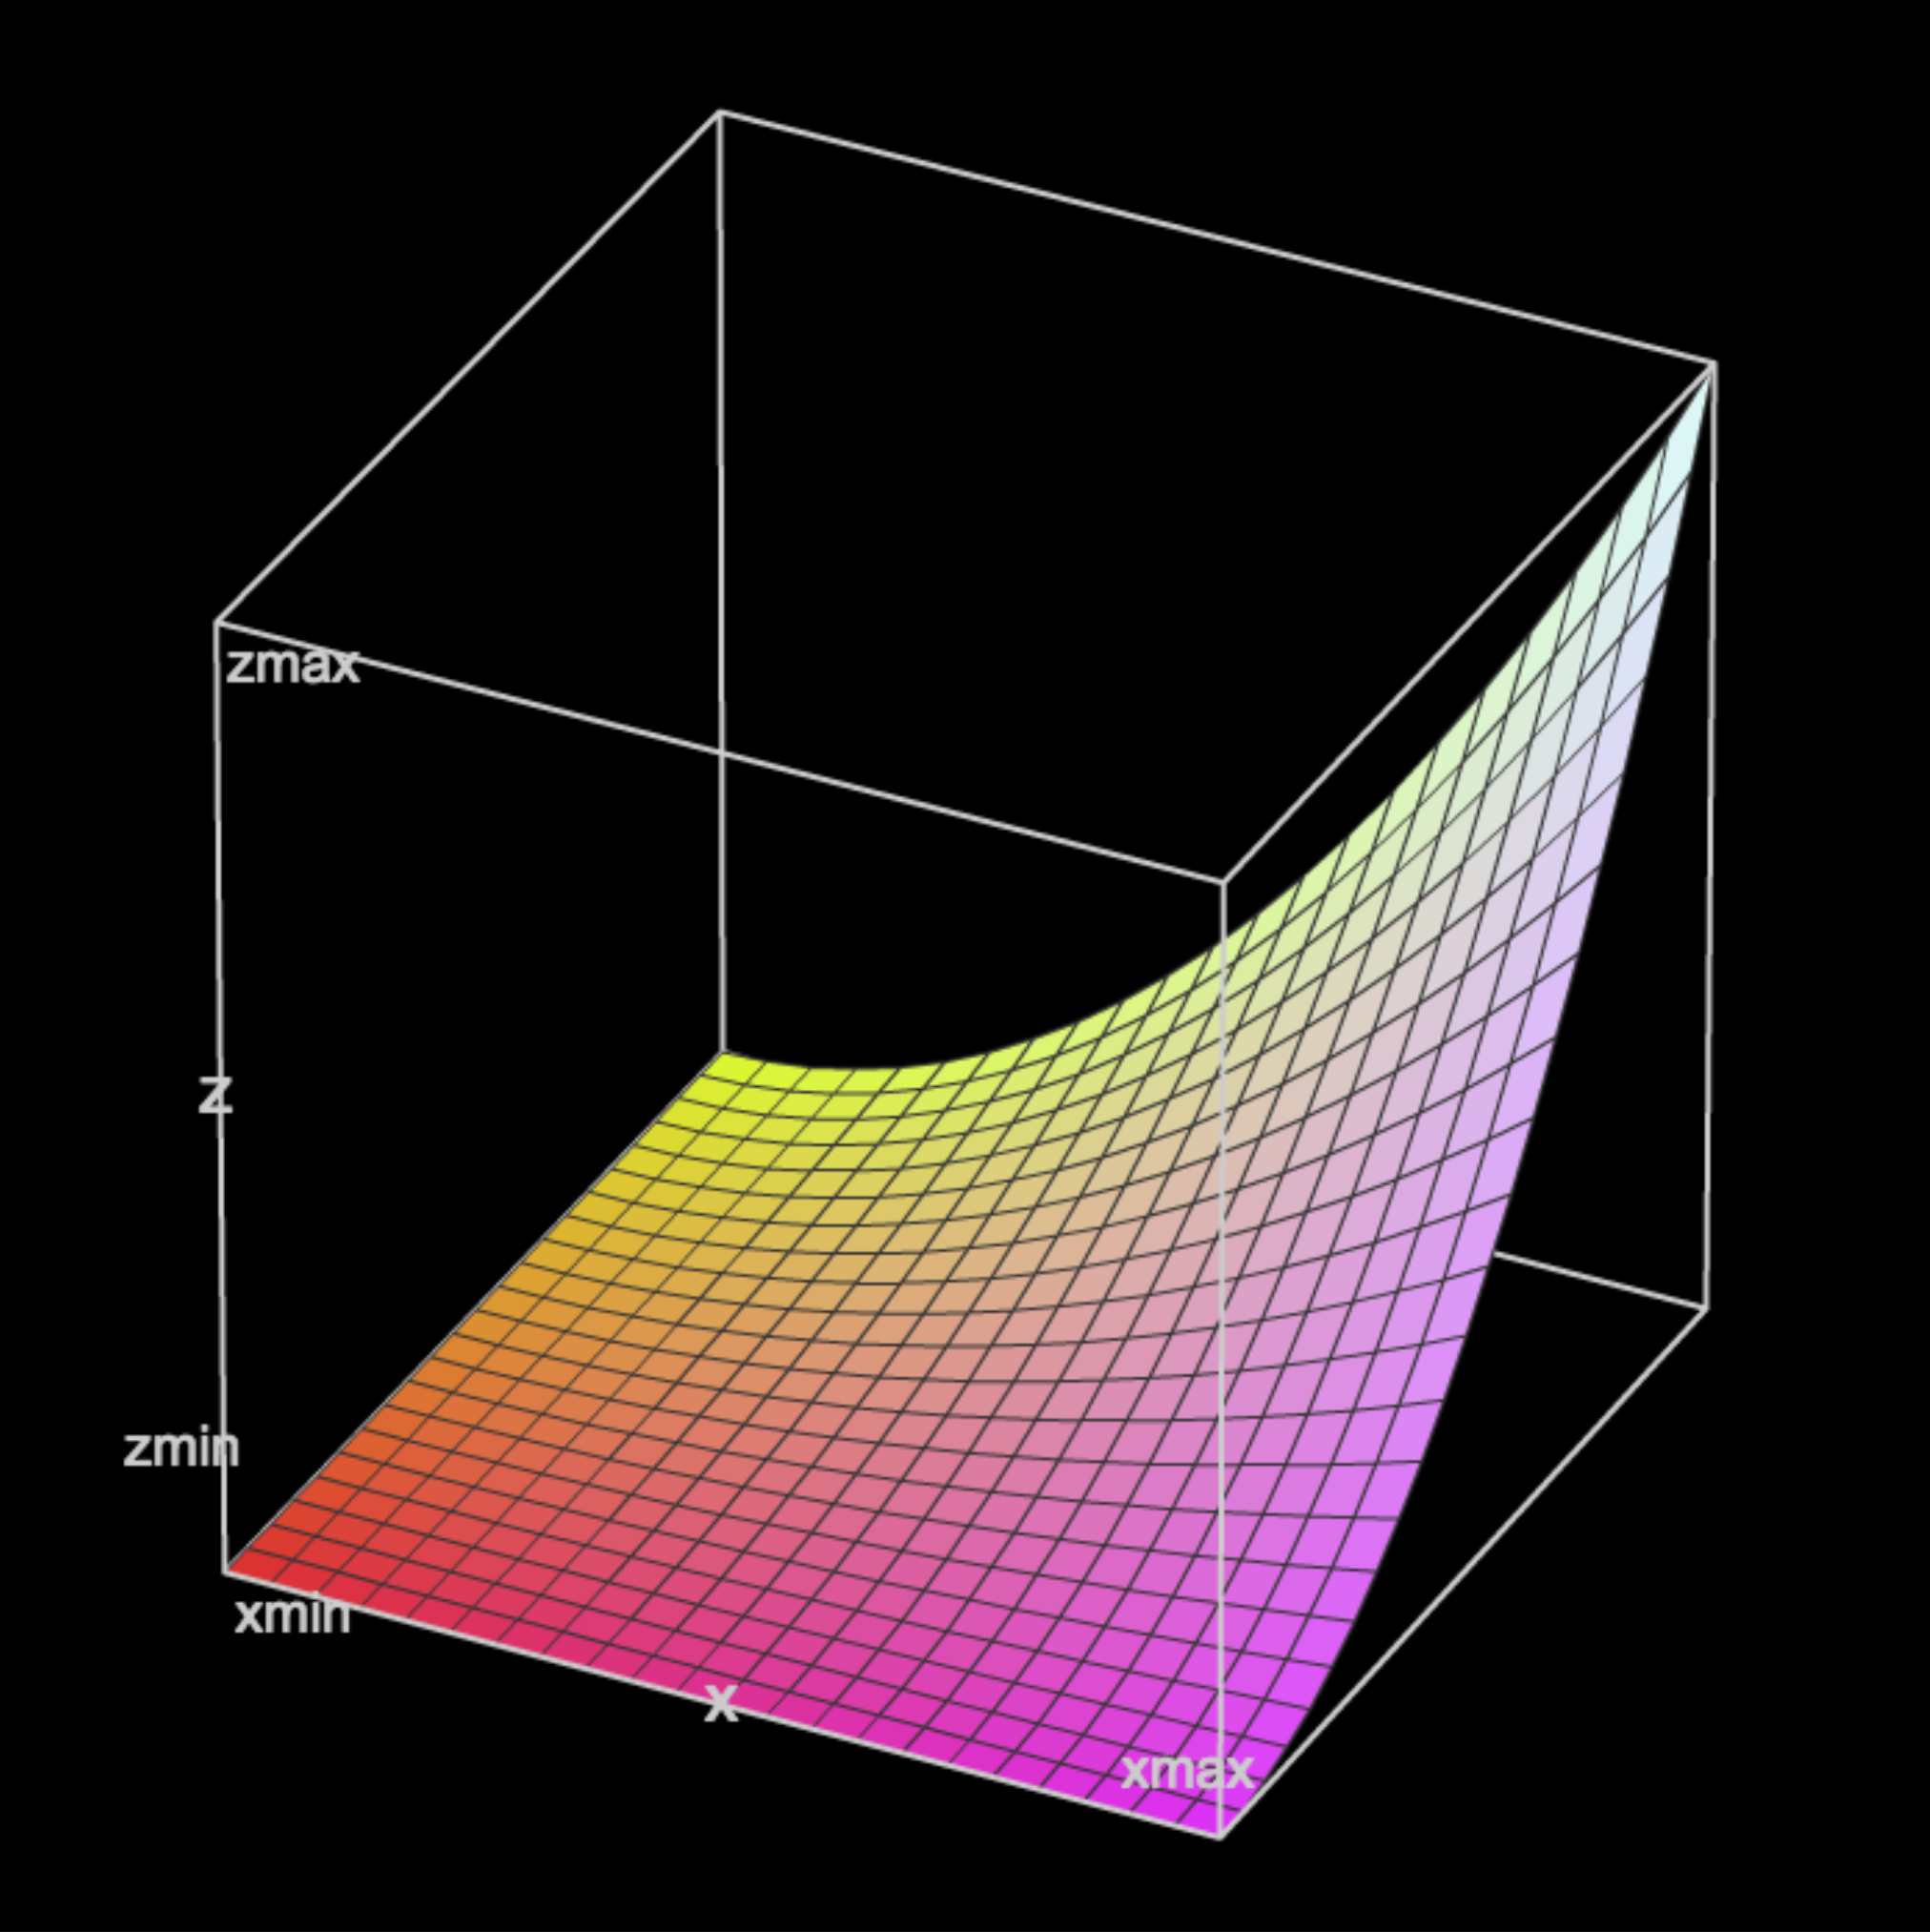
\includegraphics[width=0.8\linewidth]{squared-3b}
    \caption{Función cuadrática, ecuación~\ref{eq:sqr}}
    \label{fig:squared3}
\end{figure}

% FIGURA DE FUNCIÓN EULER
\begin{figure}[p]
    \centering
    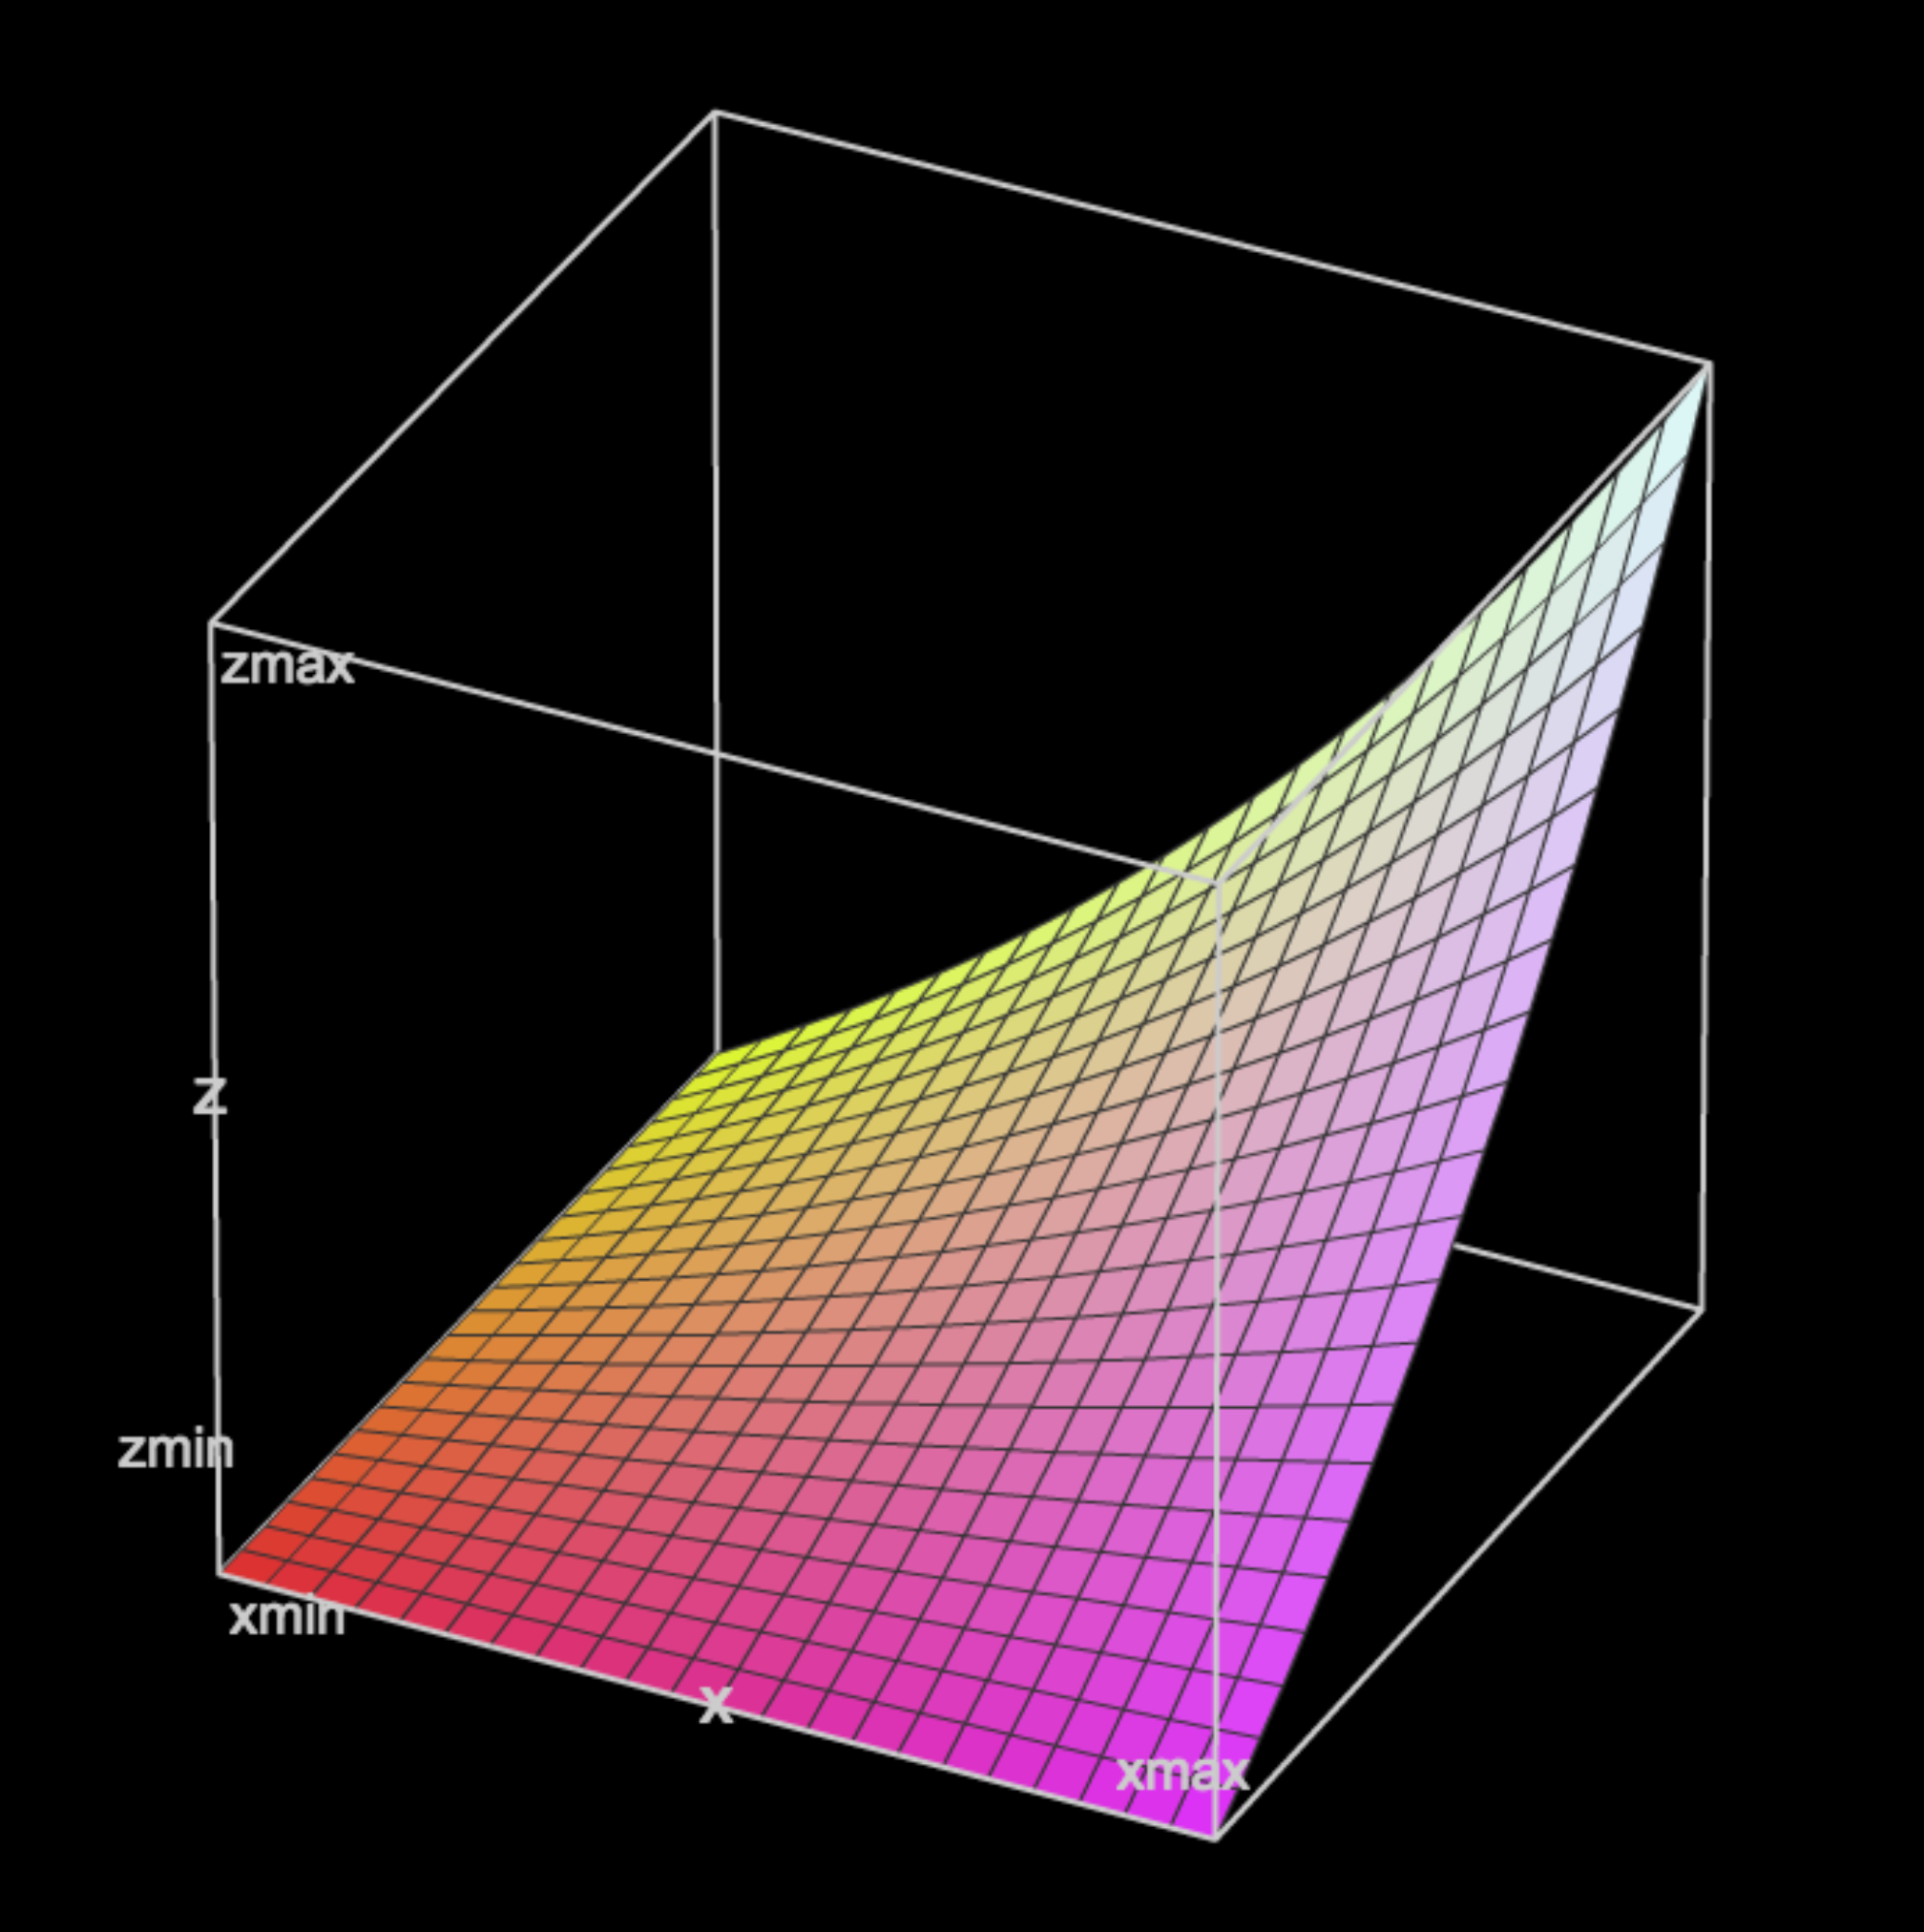
\includegraphics[width=0.8\linewidth]{euler-3b}
    \caption{Función exponencial, ecuación~\ref{eq:exp}}
    \label{fig:euler3}
\end{figure}

\section{Metaheurísticas a implementar}
En esta sección se hablará de las metaheurísticas que fueron implementadas con sus respectivas modificaciones para tratar el problema de selección de instancia. A continuación se hablará de búsqueda local (LS), búsqueda local iterada (ILS), GRASP, y algoritmos evolutivos como GGA y SGA.
\subsection{Búsqueda local (LS)}\label{sect:ls}

La búsqueda local consiste en partir de una solución inicial, que va a ser modificada por un operador de vecindad que genera otra solución factible. Luego, la solución actual se compara con la solución generada a través de una función de evaluación de calidad, y se desecha la peor de ambas para recurrir en el mismo proceso con la restante.

Como fue descrito en la sección~\ref{sect:meta}, se tomó la representación de \textbf{SP}y \textbf{UP} para las soluciones y las funciones de evaluación se tomaron las funciones~\ref{eq:sqr}, ~\ref{eq:weight} y~\ref{eq:exp}, .

Para ~\ref{eq:exp}, $\beta$ tomó el valor del número de \textit{Euler} por la forma en que la función exponencial crece. Como se puede ver en la figura~\ref{fig:euler3}, la misma penaliza a los valores más bajos, pues su crecimiento en ese punto es lento y a medida que los valores suben, el valor de la función crece de forma más violenta. En las figuras~\ref{fig:squared3} y~\ref{fig:weighted3} se puede notar que~\ref{eq:sqr} y~\ref{eq:weight} tienen un comportamiento parecido a~\ref{eq:exp} pero menos pronunciado.

Por otra parte, el operador de vencidad que se definió consiste en una función que intercambia $K$ instancias entre \textbf{SP} y \textbf{UP} para generar nuevas soluciones, donde $K$ es un parámetro a calibrar dependiendo del problema de clasificación.

Para la selección de las instancias a intercambiar, se tomaron en cuenta dos estrategias:

\begin{itemize}
    \item \textbf{Selección aleatoria:} Se seleccionan puntos de forma aleatoria de alguno de los dos conjuntos \textbf{SP} o \textbf{UP}.
    \item \textbf{Selección en base a costos:} Las instancias a intercambiar entre \textbf{SP} y \textbf{UP} son seleccionadas dependiendo de cuánto mejoren o empeoren la solución actual. Para determinar dicha medida, se define el \textit{costo incremental} $C(e)$ como una estimación del porcentaje de mejora a la solución al insertar la instancia $e$ a la misma y el \textit{costo decremental} $D(e)$ como una estimación de mejora a la solución al extraer la instancia $e$ de la misma.

    Para el caso específico de IS/PS, se tomaron dos definiciones de las función de costo incremental y decremental.

    \begin{itemize}
        \item \textbf{Prueba por fuerza bruta:} En el caso de la función incremental $C(e)$, el valor se obtiene con la diferencia entre la evaluación de la calidad de la solución que contiene al punto $e$ y la evaluación de la calidad de la solución que no contiene al punto $e$. Y en el caso de la función decremental $D(e) = -C(e)$.

        \item \textbf{Variación de posición del centroide:} En este caso se define la función incremental $C(e)$ como la variación de la posición del centroide de la clase de $e$, cuyo valor se considera mejor si es mayor. Y definimos la función decremental $D(e)$ igual que $C(e)$ pero en este caso su valor se considera mejor mientras sea menor.
    \end{itemize}

    La estrategia por fuerza bruta es la más convencional de las dos, puesto que obtiene el costo a partir de la función de evaluación definida para la búsqueda local y por ende asegura que la perturbación mejore la solución anterior. Pero por otro lado, se trata de un algoritmo con un orden de ejecución alto para la cantidad de veces que se podría repetir.

    La estrategia de la distancia al centroide se trata de insertar puntos a la solución que modifiquen de una manera significativa la posición del centroide actual. Esto es porque una instancia que no modifique la posición del centroide de forma significativa, es una instancia cuyo valor no influye tanto a la hora de clasificar.
\end{itemize}

\begin{algorithm}
    \DontPrintSemicolon
    \vspace*{0.1cm}
    \KwIn{SP, UP : Conjunto de puntos, K : Entero}
    \KwOut{SP', UP'}
    \ForEach{$1 \dots K$}{
        $sacar \leftarrow booleano\_al\_azar()$\;
        \If{$sacar$}{
            $punto \leftarrow punto\_al\_azar(SP)$\;
            $SP' \leftarrow SP\ \backslash{}\ \{punto\}$\;
            $UP' \leftarrow UP\ \cup\ \{punto\}$\;
        }
        \Else{
            $punto \leftarrow punto\_al\_azar(UP)$\;
            $UP' \leftarrow UP\ \backslash{}\ \{punto\}$\;
            $SP' \leftarrow SP\ \cup\ \{punto\}$\;
        }
    }
    \vspace*{0.1cm}
    \caption{Operador de vecindad con selección aleatoria}
\end{algorithm}

\begin{algorithm}
    \DontPrintSemicolon
    \vspace*{0.1cm}
    \KwIn{SP, UP : Conjunto de puntos}
    \KwOut{SP', UP'}
    \ForEach{$1 \dots K$}{
        $sacar \leftarrow booleano\_al\_azar()$\;
        \If{$sacar$}{
            $punto = argmin\{C(e) | e \in SP\}$\;
            $SP' \leftarrow SP\ \backslash{}\ \{punto\}$\;
            $UP' \leftarrow UP\ \cup\ \{punto\}$\;
        }
        \Else{
            $punto = argmax\{C(e) | e \in UP\}$\;
            $UP' \leftarrow UP\ \backslash{}\ \{punto\}$\;
            $SP' \leftarrow SP\ \cup\ \{punto\}$\;
        }
    }
    \vspace*{0.1cm}
    \caption{Operador de vecindad con selección en base a costos}
\end{algorithm}

\subsection{Búsqueda local iterada (ILS)}
La búsqueda local iterada se trata de realizar una búsqueda local sobre una solución inicial para obtener una mejor solución, la cual se perturba para generar una nueva solución inicial que se utiliza para realizar el mismo proceso. La solución perturbada puede ser mejor o peor que la solución generada por la búsqueda local, dado que lo que se quiere obtener al realizar dicha perturbación es expandir el espacio de búsqueda (lo que puede generar una solución peor pero que al realizar la búsqueda local sobre ella, lleve a un valor mejor que el encontrado) o mejorar aún más la solución actual.

En los experimentos a realizar en esta metaheurística se tomaron en cuenta 2 formas de perturbación de soluciones:

\begin{itemize}
    \item [\textbf{Perturbación aleatoria}:] Se perturba de forma aleatoria pero reservada, es decir, sólo se cambia una pequeña cantidad de atributos al azar de la solucion a perturbar para que la misma se mantenga en la misma localidad.
    \item [\textbf{Perturbación \textit{Greedy}}:] Se perturba la solución con un algoritmo \textit{Greedy} como \textit{CNN }o \textit{MCNN}, los cuales generan soluciones aleatorias que pueden tener una cantidad de cambios considerables. Esta perturbación puede generar soluciones incluso peores que la inicial, pero que diversifica el espacio de búsqueda para acceder a otras localidades.
\end{itemize}

La idea detrás de estos tipos de perturbación es mejorar las soluciones que se puedan encontrar con el algoritmo. Una vez ejecutada una búsqueda local, existen dos escenarios posibles: El primero es que la búsqueda no llegó a generar el mejor valor local, para lo cual se ejecuta el primer tipo de perturbación intentando así alcanzarlo. Y el segundo es que la búsqueda local sí consiguipo el mejor valor local, por lo que es necesario salir del mismo para ampliar el espacio de búsqueda cayendo en otra localidad de búsqueda y para ello se ejecuta el segundo tipo de perturbación. Para una referencia visual, ver la figura~\ref{fig:perturbaciones}.

% FIGURA DE TIPOS DE PERTURBACIÓN
\begin{figure}[h!]
    \centering
    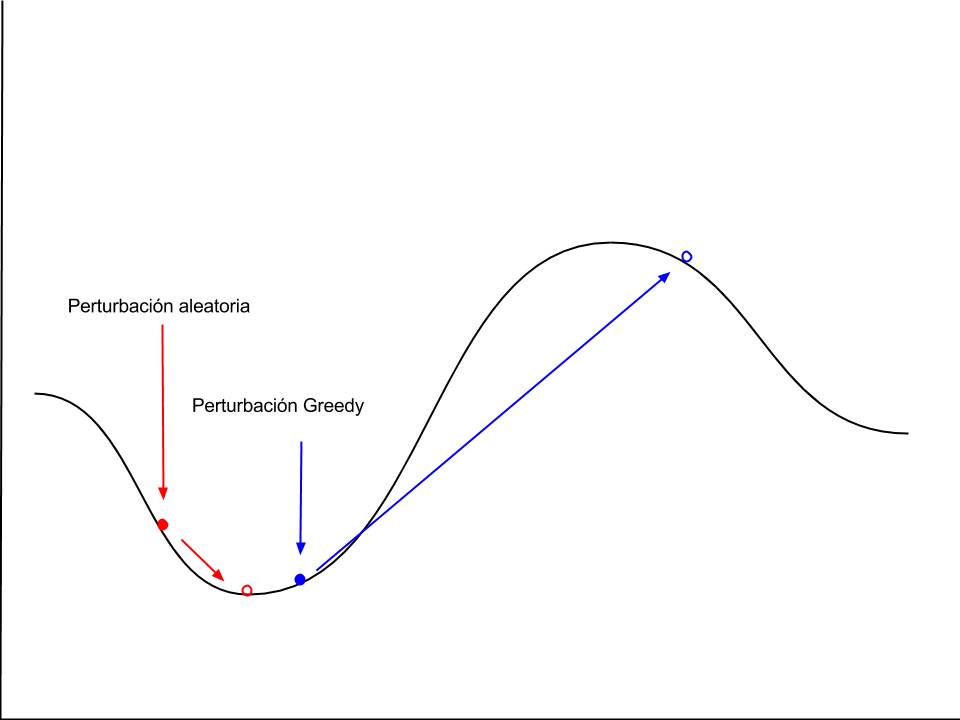
\includegraphics[width=\linewidth]{perturbaciones}
    \caption{Ejemplo de tipos de perturbación. Rojo: Perturbación aleatoria y resultado, Azul: Perturbación Greedy y resultado}
    \label{fig:perturbaciones}
\end{figure}

\subsection{\textit{\textbf{Greedy Randomized Adaptive Search Procedures}} (GRASP)}

GRASP (por sus siglas en inglés \textit{Greedy Randomized Adaptive Search Procedures}) es una metaheurística de trayectoria que hace uso de un algoritmo \textit{Greedy} aleatorio para generar soluciones diversas y de esta forma recorrer la mayor cantidad de vecindades del espacio de búsqueda. En cada iteración se hace uso de dicho algoritmo para generar una solución aleatoria y luego a esta se le aplica una búsqueda local para intentar mejorarla (Véase el algoritmo~\ref{alg:grasp}). Cabe destacar que toda solución es generada desde cero y no depende de ninguna solución anterior, por lo que se pueden explorar distintas vecindades y llegar a un mejor resultado.

\begin{algorithm}
    \DontPrintSemicolon
    \vspace*{0.1cm}
    \KwIn{N, Semilla : Entero}
    \KwOut{$S_{best}$}

    $f_{best} \leftarrow \infty$\;
    \ForEach{$1 \dots N$}{
        $S \leftarrow AlgoritmoGreedyAleatorio(Semilla)$\;
        $S \leftarrow BusquedaLocal(S)$\;
        \If{$f(S) < f_{best}$}{
            $S_{best} \leftarrow S$\;
            $f_{best} \leftarrow f(S)$\;
        }
    }
    \vspace*{0.1cm}
    \caption{Algoritmo GRASP}
    \label{alg:grasp}
\end{algorithm}
La implementación en general es simple, pero lo que hace que sea efectivo o no es la generación de las soluciones aleatorias. La función que realiza esta tarea define un costo incremental para cada punto dentro del conjunto \textbf{UP} para decidir cuál ellos es el mejor candidato para ser añadido a la solución \textbf{SP}. En el caso de IS/PS, se tomó la función \textit{Variación de posición del centroide} definida en la sección~\ref{sect:ls}. Véase el algoritmo~\ref{alg:greedy-random-grasp} para más información.


\begin{algorithm}
    \DontPrintSemicolon
    \vspace*{0.1cm}
    \KwIn{Semilla : Entero}
    \KwOut{$S_{best}$}

    $Candidatos \leftarrow ConjuntoAleatorio()$\;
    $EvaluarCostoIncremental(e)|\forall e\in Candidatos$\;
    \While{$Candidatos\neq \emptyset$}{
        $C_{min} \leftarrow min\{C(e) | e \in C\}$\;
        $C_{max} \leftarrow max\{C(e) | e \in C\}$\;
        $RCL \leftarrow \{e\in C|C(e)\leq C_{min} +\alpha (C_{max} - C_{min})\}$\;
        $s \leftarrow Aleatorio(RCL)$\;
        $S_{best} \leftarrow S_{best}\cup \{s\}$\;
        $Candidatos \leftarrow Candidatos\setminus \{s\}$\;
        $EvaluarCostoIncremental(e)|\forall e\in Candidatos$\;
    }
    \vspace*{0.1cm}
    \caption{Algoritmo Greedy Aleatorio}
    \label{alg:greedy-random-grasp}
\end{algorithm}


\subsection{Algoritmos evolutivos}
Los algoritmos genéticos son metaheurísticas que hacen alusión a la metáfora de la evolución biológica natural. Hacen uso del concepto de población de individuos (los cuales representan soluciones potenciales al problema) que luego son sometidos a operadores como la selección, la recombinación y la mutación para evolucionar los individuos de dicha población, es decir, mejorar las soluciones que estos representan. Más específicamente:

\begin{itemize}
\item \textbf{Mutación}: Se trata de un operador cuya función principal es aportar nueva información a la población al modificar los genes de las soluciones intermedias y de esta manera poder explorar diferentes espacios de búsqueda. El mismo simula la aparición de nuevos genes en la población que aumentan la posibilidad de supervivencia.

\item \textbf{Recombinacion/Cruce}: Este operator permite el intercambio de información entre dos o más individuos de la población para generar unos o más individuos hijos. Simula la reproducción de los invididuos.

\item \textbf{Selección}: Este operador permite definir qué individuos van a participar en la recombinación o cruce y a su vez, los genes que pasarán a las siguientes generaciones. Simula el proceso de selección natural.
\end{itemize}

En nuestor caso particular, la mutación consiste en perturbar la solución que representa el individuo $n$ veces, la selección es completamente aleatoria, y la recombinación/cruce es XXX INSERTAR DESCRIPCION DE RECOMBINACION/CRUCE XXX

El esquema más tradicional que define el uso de estos operadores son los \textit{Algoritmos Genéticos}. A continuación se definen dos algoritmos: GGA y SGA

\subsubsection{Algoritmo Genético Generacional (GGA)}

Este algoritmo es el más apegado a la metáfora evolutiva. El mismo parte de una población de tamaño $n$ para generar una población descendente tomando el mejor individuo entre ellas como solución. Esto lo hace seleccionando dos individuos de la población original para cruzarlos y generar dos hijos que formarán parte de la población hija, repitiendo este proceso hasta que la misma alcance el mismo tamaño que su predecesora. Ver algoritmo~\ref{alg:gga}


\begin{algorithm}[!h]
    \DontPrintSemicolon
    \vspace*{0.1cm}
    \KwIn{n tamaño de la población, cp probabilidad de cruce, mp probabilidad de mutación}
    \KwOut{Solución al problema}

	$P \leftarrow $ Generar solución aleatoria de $n$ individuos\;
	$s^{*} \leftarrow $ mejor individuo de P\;
    \While{$\neg $ Condición de parada}{
    		$P^{'} \leftarrow \emptyset$\;
    		\While{$\left\vert P^{'}\right\vert < n$}{
    			$p1 \leftarrow $ Seleccionar un individuo en $P$\;
    			$p2 \leftarrow $ Seleccionar un individuo en $P$\;
    		   $c1,c2 \leftarrow $ recombinar $p1$ y $p2$ con probabilidad cp\;
    		   Mutar $c1$ y $c2$ con probabilidad mp\;
    		   $P^{'} \leftarrow P^{'} \cup \{c1,c2\}$\;
    		   }
    		   $P \leftarrow P^{'}$\;
    		   \If{El mejor individuo en P es mejor que $s^{*}$}{
				$s^{*} \leftarrow $ el mejor individuo en P\;    		   
    		   }
    		   

    }
	\Return $s^{*}$    
    \vspace*{0.1cm}
    \caption{Algoritmo Genético Generacional}
    \label{alg:gga}
\end{algorithm}
  
\subsubsection{Algoritmo Genético Estacionario (GGA)}

Como se dice en ~\cite{whitley1988genitor}, SGA (\textit{Steady-State Genetic Algorithm}) es un enfoque distinto en el esquema de los algoritmos evolutivos dado que el mismo no sigue un esquema generacional en el que se genera una nueva población en cada paso del algoritmo. SGA comienza con una población de tamaño $n$ y en cada iteración se produce un máximo de dos nuevos individuos, y no una población completa como lo hace GGA.

En cada iteración se eligen dos individuos padres mediante el operador de selección, se generan uno o dos hijos mediante el cruce, se mutan a través del operador de mutación y finalmente se sigue una estrategia de selección para reemplazar uno o dos individuos de la población actual por la nueva descendencia, lo que mantiene el tamaño $n$ de la población. Ver algoritmo~\ref{alg:sga}


\begin{algorithm}[!h]
    \DontPrintSemicolon
    \vspace*{0.1cm}
    \KwIn{n tamaño de la población, cp probabilidad de cruce, mp probabilidad de mutación}
    \KwOut{Solución al problema}

	$P \leftarrow $ Generar solución aleatoria de $n$ individuos\;
	$s^{*} \leftarrow $ mejor individuo de P\;
    \While{$\neg $ Condición de parada}{
		$p1 \leftarrow $ Seleccionar un individuo en $P$\;
		$p2 \leftarrow $ Seleccionar un individuo en $P$\;
    	    $c1,c2 \leftarrow $ recombinar $p1$ y $p2$ con probabilidad cp\;
		Mutar $c1$ y $c2$ con probabilidad mp\;
    	    Reemplazar dos individuos en P por c1 y c2 según algún criterio\;

		\If{El mejor individuo en P es mejor que $s^{*}$}{
			$s^{*} \leftarrow $ el mejor individuo en P\;    		   
    		}
    }
	\Return $s^{*}$    
    \vspace*{0.1cm}
    \caption{Algoritmo Genético Estacionario}
    \label{alg:sga}
\end{algorithm}
\section{Evaluación experimental}
En esta sección se hablará de la configuración usada sobre los experimentos para probar y comparar las metaheurísticas búsqueda local, búsqueda local iterada, GRASP, GGA y SGA y de los resultados arrojados por las mismas.

\subsection{Conjunto de datos}

Un factor importante para la evaluación de las diferentes metaheurísticas es el conjunto de datos a utilizar, la distribución de los datos, el número de instancias, el número de atributos de cada una de ellas y la cantidad de datos ruidosos ya que los mismos influyen en el espacio de búsqueda y por ende en la efectivdad del algoritmo. 

Los conjuntos de datos usados para estos experimentos pertenecen originalmente a \textit{UCI Machine Learning Repository}~\cite{Lichman:2013} pero se obtuvo una modificación de los mismos basada en la estrategia de validación cruzada en 10 grupos (10-\textit{fold} \textit{cross-validation}) del \textit{KEEL Data-Mining Software Tool}~\cite{alcala2010keel}. Se usaron 6 conjuntos para realizar dichas evaluaciones, separando los datos en tres grupos según el número de instancias. En el cuadro~\ref{table:small-dataset} se puede ver con más detalle los conjunto de datos pequeños, en el cuadro~\ref{table:medium-dataset} los medianos y en el cuadro~\ref{table:large-dataset} los grandes.

\begin{table}[!h]
	\centering
	\begin{tabular}{c c c c}
	\hline
	Conjunto & Instancias & Atributos & Clases \\
	\hline
	Glass & 214 & 9 & 7 \\
	Iris & 150 & 4 & 3 \\
	\end{tabular}
	\caption{Conjunto de datos pequeños}
	\label{table:small-dataset}
\end{table}

\begin{table}[!h]
	\centering
	\begin{tabular}{c c c c}
	\hline
	Conjunto & Instancias & Atributos & Clases \\
	\hline
	Australian & 690 & 14 & 2 \\
	WDBC & 596 & 30 & 2 \\
	Pima & 768 & 8 & 2 \\
	\end{tabular}
	\caption{Conjunto de datos mediano}
	\label{table:medium-dataset}
\end{table}


\begin{table}[!h]
	\centering
	\begin{tabular}{c c c c}
	\hline
	Conjunto & Instancias & Atributos & Clases \\
	\hline
	Abalone & 4174 & 8 & 28 \\
	\end{tabular}
	\caption{Conjunto de datos grande}
	\label{table:large-dataset}
\end{table}

\subsection{Parámetros}
En las diferentes metaheurísticas hay parámetros que regulan el proceso de búsqueda que realizan. Los valores dados a cada parámetro y la combinación entre ellos determinará el comportamiento y el desempaño de cada algoritmo y por lo tanto estos son altamente dependientes del problema a resolver. Esto hace que la regulación de estos parámetros no sea un proceso trivial y que conlleve un análisis con pruebas sobre los mismos para asegurar el mejor desempeño.

	Para el caso de la evaluación de las metaheurísticas descritas anteriormente, se realizó una entonación de los parámetros. En la tabla~\ref{table:parameters} se muestra los parámetros usados.  

\begin{table}[!h]
	\centering
	\begin{tabular}{c c c c c c}
	\hline
	Parámetro & LS & ILS & GRASP & GGA & SGA \\
	\hline
	Iteraciones & 1000 & 1000 & 1000 & 1000 & 1000 \\
	Iteraciones LS & - & 100 & 100 & - & - \\
	\textit{Classification rate} & 0.9 & 0.9 & 0.9 & 0.9 & 0.9 \\
	\textit{Greediness rate} & - & - & 0.5 & - & - \\
	Población & - & - & - & 50 & 50 \\
	Prob. de cruce & - & - & - & 1.0 & 1.0 \\
	Prob. de mutación & - & - & - & XXX & XXX \\
	N perturbaciones & - & - & - & XXX & XXX \\
	\end{tabular}
	\caption{Conjunto de datos pequeños}
	\label{table:parameters}
\end{table}


\subsection{Resultados}
%\section*{Conclusiones}
%---------------------------- Bibliography -------------------------------

% Please add the contents of the .bbl file that you generate,  or add bibitem entries manually if you like.
% The entries should be in alphabetical order
\small
\bibliographystyle{abbrv}
\bibliography{informe}

% \newpage
% \section*{Apéndice}

\end{document}
